\documentclass{article}
\usepackage[utf8]{inputenc}
\usepackage[a4paper, left=1cm, right=1cm, top=1cm]{geometry}
\usepackage{tikz}
\usetikzlibrary{positioning,shadings}
\usetikzlibrary{arrows}
\begin{document}
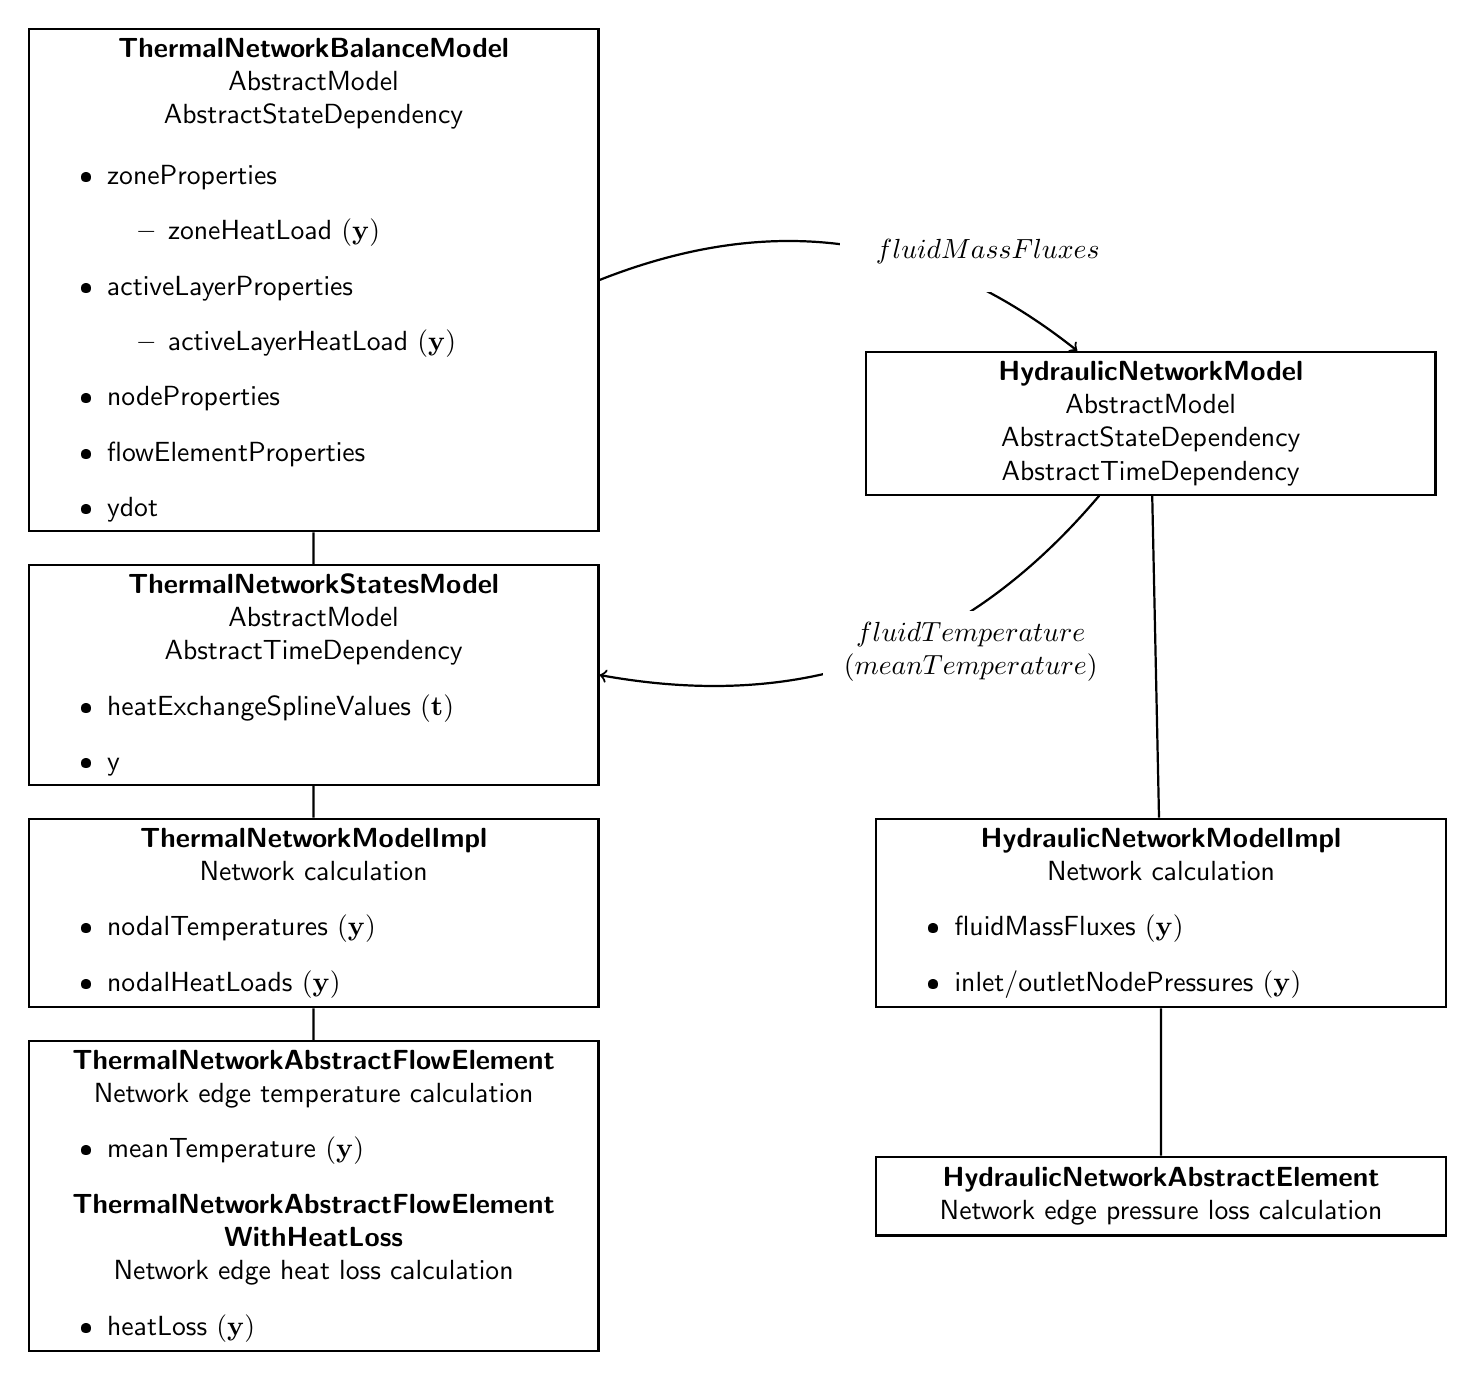
\begin{tikzpicture}[auto, node distance = 0.4cm, thick,
  every node/.style = {rectangle, font = \sffamily, draw=black,
    top color = white, bottom color = white,
    text width = 7cm, align = center, minimum height = 1cm}]
  \node (TB)                                 {\textbf{ThermalNetworkBalanceModel}\\AbstractModel\\ AbstractStateDependency\\ 
  \begin{itemize} 
  \item zoneProperties\begin{itemize}\item zoneHeatLoad  $\mathbf{(y)}$\end{itemize} 
  \item activeLayerProperties \begin{itemize} \item activeLayerHeatLoad  $\mathbf{(y)}$\end{itemize}
  \item nodeProperties 
  \item flowElementProperties 
  \item ydot 
  \end{itemize}};
  \node (TS)   [below = of TB]          {\textbf{ThermalNetworkStatesModel}\\AbstractModel\\AbstractTimeDependency \begin{itemize} \item heatExchangeSplineValues  $\mathbf{(t)}$\item y \end{itemize}};
  \node (TNImpl) [below = of TS]  {\textbf{ThermalNetworkModelImpl}\\ Network calculation\begin{itemize} \item nodalTemperatures $\mathbf{(y)}$ \item nodalHeatLoads  $\mathbf{(y)}$\end{itemize}};
  \node (TNElem) [below = of TNImpl]  {\textbf{ThermalNetworkAbstractFlowElement}\\ Network edge temperature calculation\begin{itemize} \item meanTemperature  $\mathbf{(y)}$\end{itemize}
  \textbf{ThermalNetworkAbstractFlowElement}\\ \textbf{WithHeatLoss}\\Network edge heat loss calculation
  \begin{itemize}\item heatLoss  $\mathbf{(y)}$\end{itemize}};

  \coordinate [right = 7.0cm of TNImpl] (Mitte);
  \coordinate [right = 0cm of TB] (TBright);
  \coordinate [right = 0cm of TS] (TSright);
  \node (HN)   [above = 5.3cm of Mitte]          {\textbf{HydraulicNetworkModel}\\AbstractModel\\AbstractStateDependency\\AbstractTimeDependency }; 
  \node (HNImpl)   [right = 3.5cm of TNImpl]          {\textbf{HydraulicNetworkModelImpl}\\
  Network calculation
  \begin{itemize}  \item fluidMassFluxes  $\mathbf{(y)}$\item inlet/outletNodePressures  $\mathbf{(y)}$\end{itemize}}; 
  \node (HNElem)   [right = 3.5cm of TNElem]          {\textbf{HydraulicNetworkAbstractElement}\\Network edge pressure loss calculation}; 

 \draw [black,thick]
    (TB)    --  (TS)  --  (TNImpl)  -- (TNElem)
    (HN)   --  (HNImpl) -- (HNElem);
  \path[->]  
  (TBright) edge[bend left=30] node[pos=0.8,above,draw=white,text width=3.5cm] {$fluidMassFluxes$}  (HN);
   \path[->] 
  (HN) edge[bend left=30] node[pos=0.3,below,draw=white,text width=3.5cm] {$fluidTemperature$\\$(meanTemperature)$}  (TSright);

\end{tikzpicture}\newline\newline\newline
\textbf{Variables:}
\begin{itemize}
\item $\mathbf{(y)}$ - calculated in $update()$
\item $\mathbf{(t)}$ - calculated in $setTime()$
\end{itemize}
\end{document}